\chapter{Architecture}
\label{chapter:architecture}

Alcaudon's architecture will be described in this chapter following a top-down
approach. Firstly, a general description of the different components of the system
will be explained. Finally, each of the components will be described more thoroughly.

\section{General description}

Alcaudon's platform is composed by 3 main units.

\begin{itemize}
\item \textbf{Alcaudon library}: This is the main interface between users
  and the system. In order to use Alcaudon it is necessary to have access to a
  cluster with a coordinator and computing nodes. This interface is provided as
  a library containing the tools to build dataflows, the interfaces to implement
  user defined stream computations and the tools to connect with a particular
  cluster. Since the computations are potentially infinite, the operations
  performed against the cluster are asynchronous, returning an id associated
  with the created operation.
\item \textbf{Coordinator node}: This is the main component of the system. It
  coordinates the life cycle of the different components of the cluster such as
  the computing nodes. It is also responsible of performing the scheduling of
  the user defined dataflows given the resources provided by the computing
  nodes. Finally, it is the interface between the cluster and the users, where
  they deploy their dataflow topologies.

\item \textbf{Computing nodes}: These nodes are in charge of executing the
  actual computations provided by Alcaudon's users. These nodes take care of
  storing intermediate results published to streams. They register dynamically
  to the cluster contacting the coordinator node. A deployment can be composed
  from one computing node up to thousands, as needed. Each of these nodes
  provides certain resources to the system, known as \textit{computation slots}.
  The number of slots is configurable, but they correlate with the number of
  available CPU's in the underlying hardware.
\end{itemize}

A high level overview of the system can be seen in
figure~\ref{fig:architecture}. The majority of the parts of the system have been
modeled as Actors. As it was stated previously it is a very good fit for this
kind of applications. Where possible, object oriented design patterns\cite{gof}
such as \textbf{builder} or \textbf{factory} have been used. However, functional
programming constructs such as monads\cite{monads}, type
classes\cite{typeclasses} or Algebraic Data Types have been used more widely.

Once the different parts of the system have been presented, they will be
inspected in detail.

\begin{figure}
  \centering
  
\includegraphics[width=1\textwidth]{architecture.pdf}
  \caption{Alcaudon architecture schema}
  \label{fig:architecture}
\end{figure}

\section{Alcaudon library}

In the first place, the user facing interface will be presented in detail. In order
to create a streaming data processing pipeline, or dataflow topology as it has
been defined during all this document, users should provide their business
logic. To achieve this goal, Alcaudon provides certain interfaces so users
just need to care about their code. These interfaces are available as a library
that can be found at at Sonatype OSSRH \footnote{http://central.sonatype.org/pages/ossrh-guide.html}.

\begin{figure}
  \centering
  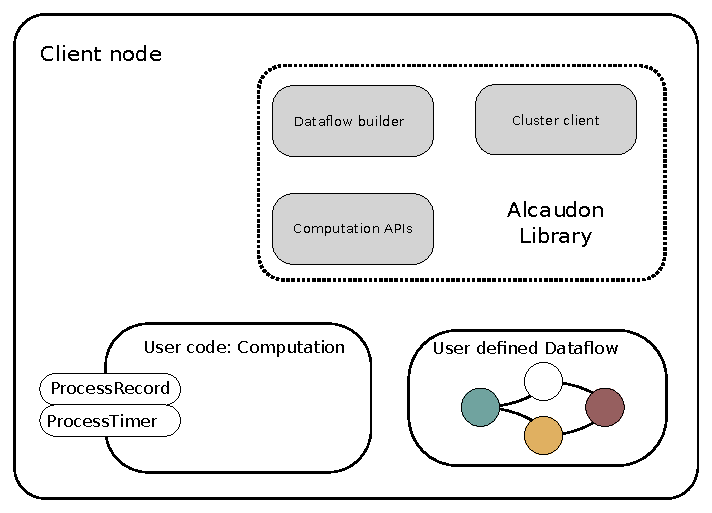
\includegraphics[width=0.6\textwidth]{client.pdf}
  \caption{Alcaudon library}
  \label{fig:library}
\end{figure}

This library is composed of three modules as it is shown in figure~\ref{fig:library}:

\begin{itemize}
\item Computation API's: Interface that users should implement in order to
  create computations.
\item Dataflow builder: This component is used to build dataflow topologies and
  later on submit the to the cluster coordinator.
\item Cluster client: Communication layer between clients and Alcaudon clusters.
  It handles all the operations needed to submit custom code to the cluster as well
  as the stream processing pipeline definition.
\end{itemize}

\subsection{Computation API's}

\begin{figure}[!h]
  \begin{center}
  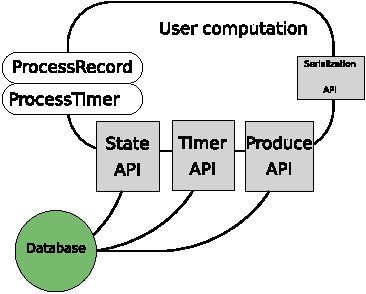
\includegraphics[width=0.5\textwidth]{libraryApi.pdf}
  \caption{Alcaudon computation API's}
  \label{fig:apis}
  \end{center}
\end{figure}

As explained before, in order to create custom computations to process unbounded
data-sets in Alcaudon, it is necessary to implement an interface. The interface
is listed in~\ref{code:computation}. This interface gives access to the
abstractions provided by the system as represented in figure~\ref{fig:apis}. As
it can be observed, there are two methods to be implemented;
\lstinline[columns=fixed]{def processRecord(record: Record): Unit} and \lstinline[columns=fixed]{def processTimer(timer: Timer): Unit}.

\begin{lstlisting}[language=scala, frame=trBL, label=code:computation, float=ht, caption = {Computation API's}]
trait Computation
    extends ProduceAPI
    with TimerAPI
    with StateAPI
    with SerializationAPI
    with RuntimeContext {
  ...
  def processRecord(record: Record): Unit
  def processTimer(timer: Timer): Unit
  ...
}
\end{lstlisting}

\begin{lstlisting}[language=scala, frame=trBL, label=code:computationExample, float=ht, caption = {Computation example}]
class Windower extends Computation {
  // Counts the number of records per key
  def processRecord(record: Record): Unit = {
    val bucketCount: Int = deserialize(get(record.key))
    set(record.key, serialize(bucketCount + 1))
    setTimer(FixedRecurrentTimer(record.key, 5.minutes))
  }

  // Timers are triggered and produce records with the count of keys.
  def processTimer(timer: Timer): Unit = {
    val bucketCount: Int = deserialize(get(timer.tag))
    produceRecord("windowsCount", RawRecord(get(timer.tag), timer.timestamp))
  }
}
\end{lstlisting}

These methods represent the main entry point into user code, hooked in reaction to
record receipt and timers expiration. These constitute the application logic.
Within the execution of these methods, Alcaudon provides different functions to
work with persistent state, publish new records to streams, set timers or
serialize arbitrary data types. In Alcaudon, each computation can subscribe to
multiple sources represented as streams. Data travels in its simplest form,
as an array of bytes. One specific example can be found in listing~\ref{code:computationExample}.

\begin{figure}
  \begin{center}
    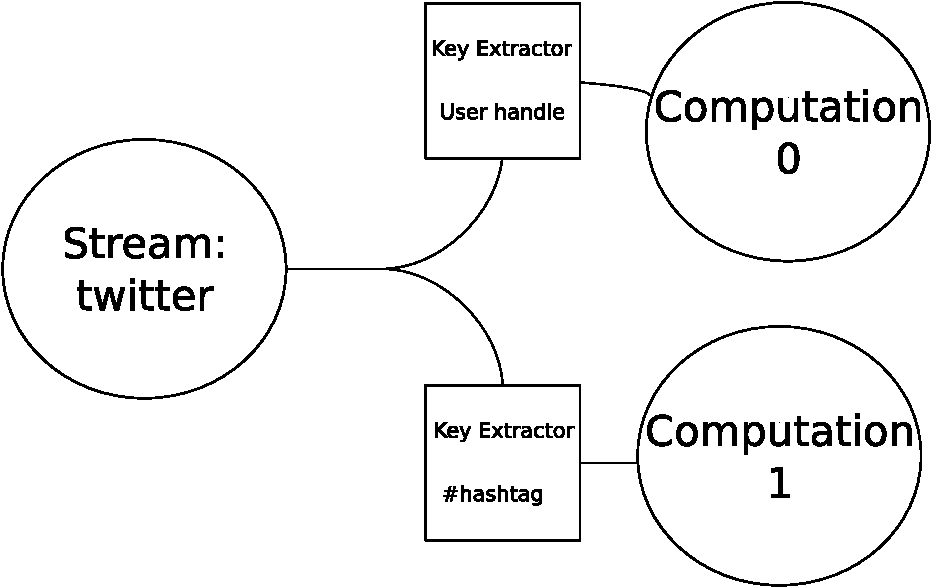
\includegraphics[width=0.5\textwidth]{keypartitioning.pdf}
    \caption{Alcaudon record key assignment}
    \label{fig:keypartitioning}
  \end{center}
\end{figure}

However, for each stream subscription users should provide a key extraction
function, this process shown in figure~\ref{fig:keypartitioning}. Having a key
per record allows the implementation of parallelization strategies such as key
partitioning. Therefore, every record emitted by one of the subscribed sources,
an instance of the class \lstinline[columns=fixed]{Record} listed
in~\ref{code:records}, will be injected with the call to
\lstinline[columns=fixed]{processRecord}.

\begin{lstlisting}[language=scala, frame=trBL, label=code:records, float=ht, caption = {Record classes}]
case class RawRecord(value: Array[Byte], timestamp: Long) {
  val id = UUID.randomUUID().toString
}
case class Record(key: String, rawRecord: RawRecord) {
  val value = rawRecord.value
  val timestamp = rawRecord.timestamp
  val id = UUID.randomUUID().toString
}
\end{lstlisting}

Timers are the other possible trigger for user defined code execution. In
Alcaudon there are three types of timers:

\begin{itemize}
\item \textit{Fixed timers}: This kind of timers are triggered once at a
  specific wall time.
\item \textit{Recurrent fixed timers}: This timer resembles the previous timers
  with the exception that it is executed recurrently. I.E., every five minutes.
\item \textit{Watermark timers}: This timer tries to estimate the point where all
  the events up to certain window have been consumed by the system and execute
  then. The mechanism and algorithm used to implement them will be explained
  later.
\end{itemize}

When a timer is executed it has as a parameter an instance of the class Timer
listed in ~\ref{code:timers}. These constructs are key to the domain of unbounded
data-sets due to their very nature. A mean to emit partial results is needed, so
this is the mechanism provided by Alcaudon to emit results.

\begin{lstlisting}[language=scala, frame=trBL, label=code:timers, float=ht, caption = {Timer class}]
  case class Timer(tag: String, timestamp: Long)
\end{lstlisting}

\subsection{Dataflow builder}

Once the computations are implemented, users need a way to build the dataflow topologies.
To achieve this goal, the system provides a dataflow builder. Using this instrument,
users are able to define dependencies among the computations in the system.
These main entities that can be used in Alcaudon are:

\begin{itemize}
  \item \textit{Sources}: Sources bring external data into the system. Some
    examples could be a TCP/IP socket, Twitter streaming API, Apache Kafka,
    Zeromq, etc.
  \item \textit{Computations}: Computations are user defined business logic.
  \item \textit{Streams}: Streams represent the delivery instrument between
    different computations in Alcaudon. Computations subscribe to one or more
    streams and publish to zero or more streams. Alcaudon guarantees the
    delivery of records along these streams.
  \item \textit{Sinks}: Sinks are a special kind of streams, providing a way to
    publish data to external systems such as http endpoints or databases. They
    are useful to project final results.
\end{itemize}

Alcaudon dataflow builder is defined in listing~\ref{code:builder}. Dependencies
are checked, thus if one computation depends or publishes into an unknown stream,
the dataflow definition will be considered invalid. Internally, defined
dataflows are represented as a \acf{DAG}~\ref{fig:dataflowbuilder}. In this graph, vertices
represent computations and streams while edges represent the dependencies
between them or how data flow along the system. Considering that the execution
of the dataflow is performed remotely and computations are arbitrary user code,
computations are represented as their fully qualified name inside the \acs{JVM}
classpath. Using this fully qualified name in combination with dynamic class
loaders, it is possible to load code dynamically. In conclusion, with this builder
it is possible to create declarative representations of Alcaudon data pipelines.
This representation abstracts away all the details about in which compute nodes
code will run or how parallelism will be implemented. This approach is quite
similar to how Free Monad\cite{freemonad}, SQL or Prolog works.

\begin{lstlisting}[language=scala, frame=trBL, label=code:builder, float=ht, caption = {Alcaudon's DataflowBuilder}]
DataflowBuilder(dataflowName: String)
  .withSource(sourceName: String, sourceDescription: SourceDescription)
  .withComputation(computationName: String,
    computation: Computation,
    outputStreams: Set[StreamID],
    AlcaudonInputStream(StreamID)(keyExtractor: Array[Byte] => String)*
  .withSink(sinkName: String, sinkDescription: SinkDescription)
  .build()
\end{lstlisting}

\subsection{Cluster client}

\begin{figure}
  \centering
  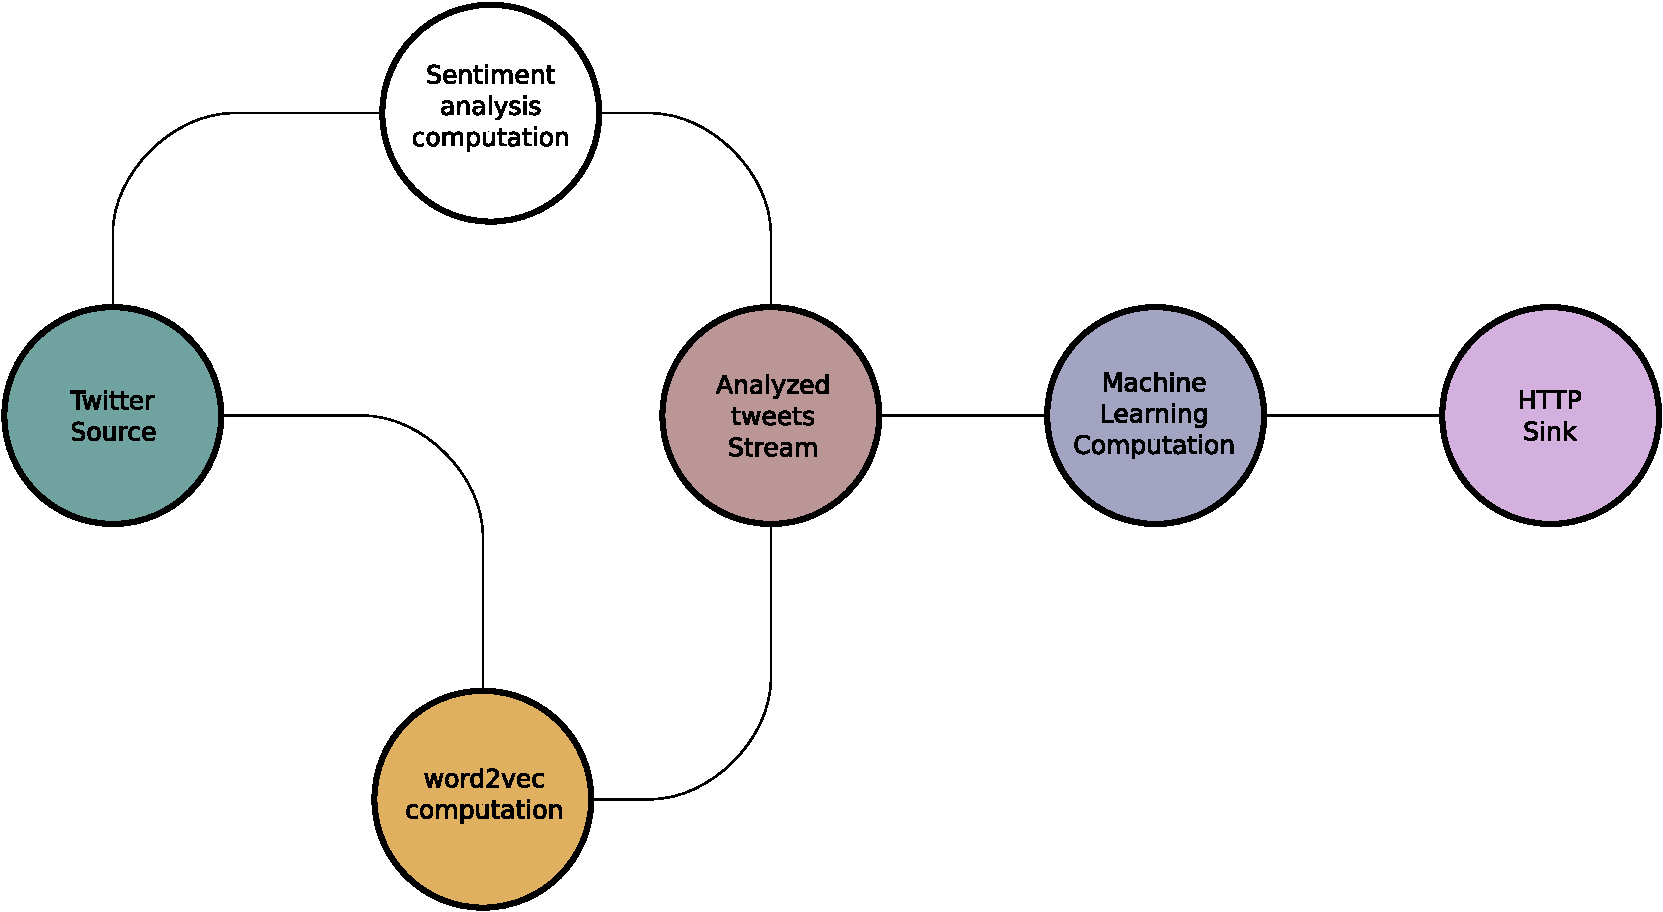
\includegraphics[width=0.8\textwidth]{dataflowbuilder.pdf}
  \caption{Dataflow \acs{DAG} example}
  \label{fig:dataflowbuilder}
\end{figure}

Once the computations and topology have been defined, some machinery is required
in order to execute them in an Alcaudon cluster
(figure~\ref{fig:dataflowbuilder}). In Alcaudon library there are the tools
needed to connect to an existing cluster and perform certain operations. The
available operations are listed in table~\ref{tab:operations}. Creating a
dataflow pipeline is an asynchronous operation, returning a DataflowPipeline
\acf{UUID} that identifies the created pipeline. With this \acs{UUID} it is
possible to perform some operations over the pipeline.

\begin{table}[hp]
\centering
\begin{tabular}{|l|l|l|}
\hline
\textbf{Action} & \textbf{Parameters} & \textbf{Returned info} \\ \hline
\begin{tabular}[c]{@{}l@{}}Send Dataflow topology\end{tabular}  & DataflowGraph and \acs{jar}s & DataflowPipeline UUID \\ \hline
\begin{tabular}[c]{@{}l@{}}Get DataflowJob execution info\end{tabular} & DataflowPipeline UUID & DatflowPipelineStatus \\ \hline
\begin{tabular}[c]{@{}l@{}}Stop DataflowJob execution\end{tabular} & DataflowPipeline UUID & DatflowPipelineStatus \\ \hline
\end{tabular}
\caption{Available cluster management operations}
\label{tab:operations}
\end{table}

In order to understand better how Alacaudon dataflow pipeline creation works, it
will be explained more thoroughly. This operation is divided into two phases,
first user code libraries are uploaded. Once the libraries are uploaded the
actual dataflow pipeline is created. Uploading user libraries is needed so
computing nodes can have access to user business logic. The number of computing nodes that
can access concurrently to these user libraries depends on the deployment,
reaching up to thousands in some cases. To avoid any scaling problems, libraries
are stored into an object storage service. In this case, they are stored in
Amazon S3\footnote{https://aws.amazon.com/s3/}. These services usually provide a
way to avoid the need to first upload the data to a backend server in order to
get access to credentials to later on upload data to an object storage services.
This is achieved using pre-signed URL's, based on a temporary token generated
using service credentials and a timestamp. In Alcaudon, cluster clients
request the creation of a dataflow pipeline. As a response, a pre-signed URL
alongside an UUID that identifies the operation is returned by the cluster
coordinator. Once cluster clients have the URL, they can use it to upload user
code directly to the object storage service. With the user code uploaded, the
next step is to create the actual Dataflow pipeline. Given the returned UUID a
request is done to cluster coordinator in order to finish the dataflow pipeline
creation. The communication is performed using akka remote that allows
communications with remote actor systems.The whole process is represented as a
sequence diagram in figure~\ref{fig:pipelinecreation}. This process is performed
transparently by the library from users perspective.

\begin{figure}[!h]
  \centering
  \scalebox{0.6}{
    \input{figures/dataflowcreation.latex}
  }
\caption{Sequence diagram for Dataflow pipeline creation}
\label{fig:pipelinecreation}
\end{figure}

\subsection{Serialization API}

Programmers are used to work with high level abstractions in order to model the
domain they are working on. As it has been described previously, records in
Alcaudon are a tuple of a key and an array of bytes. Given this fact, a way to
work with high level entities is needed. There are many options to serialize and
deserialize data available, such as JSON, Protocol Buffers, etc. Alcaudon users
are free to use the serialization format they prefer. However, to ease working
with the platform, a generic serialization library typeclass is provided. This
library is capable of, given an \acs{ADT} generate automatically serializers and
deserializers during compile time. This is possible thanks to an advanced Scala
feature, implicits resolution, and one library for generic programming,
Shapeless. \acs{ADT}s are a functional programming concept that allow data
representation in terms of \textit{products} and \textit{sums} of types. A
\textit{product} is a combination of different types $(A \& B)$. On the other
hand a \textit{sum} is an alternation of different types $(A | B)$. In Scala,
\acs{ADT} are expressed as case classes and traits as shown in
listing~\ref{code:adt}.

\begin{lstlisting}[language=scala, frame=trBL, label=code:adt, float=ht, caption = {\acs{ADT} example}]
  sealed trait Message // Message = (Tweet | Account)
  case class Tweet(user: String, id: Int, timestamp: Long) extend Message // Tweet = (String & Int & Long)
  case class Account(name: String, age: Int) extend Message // Account = (String & Int)
\end{lstlisting}

Taking this into account, case classes could be represented as lists of types,
in \lstinline[columns=fixed]{Tweet} example it can be summarized as a list of
three types, \lstinline[columns=fixed]{String & Int & Long}. Shapeless allows
to represent case classes as a \acf{HList} of types working with them
as they are regular types. Once it is possible to encode \acs{ADT}s as
\acs{HList} of types a tool to convert that generic representation into
a serializer is needed. To achieve this goal, Scala implicit type system is the
answer. Scala implicits are a way to provide certain parameters marked as
implicits to functions without the need to pass them explicitly. Scala compiler has
a set of strict rules\footnote{http://docs.scala-lang.org/tutorials/FAQ/finding-implicits.html}
to look for implicit parameters. The interesting part comes when functions with implicit
parameters use parametric polymorphism, such as Alcaudon's serialization typeclass
listed in~\ref{code:typeclass}.
\begin{lstlisting}[language=scala, frame=trBL, label=code:typeclass, float=ht, caption = {Serializer-Deserializer typeclass}]
trait TypeInfo[T] {
  def serialize(obj: T)(implicit output: DataOutput): DataOutput
  def deserialize(t: DataInput): T
}
\end{lstlisting}

It is possible to write an implicit rule that creates a
\lstinline[columns=fixed]{TypeInfo} for \lstinline[columns=fixed]{(A, B)} given
\lstinline[columns=fixed]{TypeInfo} for \lstinline[columns=fixed]{A} and
\lstinline[columns=fixed]{B}. This feature is provided by Scala implicit
resolution mechanism that works as an inductive solver. Therefore, if
\lstinline[columns=fixed]{TypeInfo} instances for every basic data type are
implemented it is possible to write rules for \acs{HList} of
\textit{products}. As a result, Scala compiler will be able to inductively
generate \lstinline[columns=fixed]{TypeInfo} instances for any \acs{ADT}
during compile time.

\begin{lstlisting}[language=scala, frame=trBL, label=code:generation1, float=ht, caption = {Serializer-Deserializer typeclass using parametric polymorphism}]
  implicit def genericObjectEncoder[A, H <: HList, O <: HList](
      implicit generic: LabelledGeneric.Aux[A, H],
      repFormat: Lazy[TypeInfo[H]],
      keys: Keys.Aux[H, O]
  ): TypeInfo[A] =
    new TypeInfo[A] {
      def serialize(v: A)(implicit output: DataOutput) = {
        repFormat.value.serialize(generic.to(v))
      }

      def deserialize(input: DataInput) = {
        generic.from(repFormat.value.deserialize(input))
      }
    }
\end{lstlisting}

Details about how rules for generic types and \acs{HList} are implemented can be
found in listings ~\ref{code:generation1} and ~\ref{code:generation}. For
objects of type T, Shapeless is used in order to obtain its encoding as an
\acs{HList}; this is done in \lstinline[columns=fixed]{genericObjectEncoder}.
With this encoding, it is possible to call the serializer for \acs{HList}s in
implicit method \lstinline[columns=fixed]{hListFormat}. In this method, using
recursive induction, a type class for each type is searched and combined, thus
creating a serializer for the \acs{HList} then for the type T.

\begin{lstlisting}[language=scala, frame=trBL, label=code:generation, float=ht, caption = {Serializer-Deserializer typeclass for \acs{HList}}]
  implicit def hListFormat[Key <: Symbol, Value, Remaining <: HList](
      implicit key: Witness.Aux[Key],
      lazyTih: Lazy[TypeInfo[Value]],
      lazyTit: Lazy[TypeInfo[Remaining]]
  ): TypeInfo[FieldType[Key, Value] :: Remaining] =
    new TypeInfo[FieldType[Key, Value] :: Remaining] {
      ...
      def serialize(hlist: FieldType[Key, Value] :: Remaining)(
          implicit output: DataOutput) = {
        val headOutput = tih.serialize(hlist.head)
        tit.serialize(hlist.tail)(headOutput)
      }

      def deserialize(input: DataInput) = {
        val head = tih.deserialize(input)
        val tail = tit.deserialize(input)
        field[Key](head) :: tail
      }
    }
\end{lstlisting}

As an interesting note, this part of the system has been tested using property
based testing\cite{quickcheck}. Using this kind of testing helped to spot
otherwise difficult bugs to detect.

\section{Computation node}

\begin{figure}[!h]
  \centering
  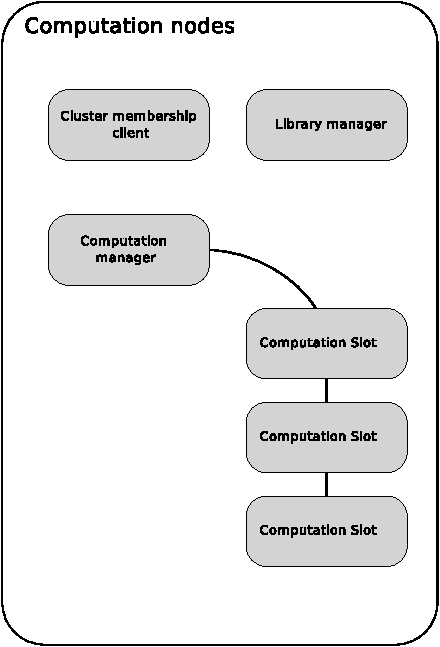
\includegraphics[width=0.5\textwidth]{computationnode.pdf}
  \caption{Computation node modules}
  \label{fig:computationnode}
\end{figure}

Once Alcaudon library has been described, computation node architecture design
will be presented. This component is in charge of executing the actual
computations. A high level overview of this component can be found in
figure~\ref{fig:computationnode}. It is composed of four modules:
\begin{itemize}
\item \textit{Cluster membership client}: This module is in charge of handling
  the communications with the cluster coordinator. It announces the availability
  of a new computing node once it is up and ready to receive work. It announces
  the intention to leave the cluster so it is possible to re-schedule work into
  other computing nodes gracefully. Another responsibility of this module is to
  send heartbeats to the cluster coordinator in order to assure that the node is
  healthy.
\item \textit{Library manager}: Library manager handles the download of user
  defined code as well as loading it into the process classpath dynamically.
  It downloads the contents from the object storage into disk, so content is
  just downloaded once per computing node. Once the \acs{jar}'s are downloaded,
  they are loaded into a controlled user \acs{JVM} classpath. This avoids
  classpath collisions, i.e. different computations use a library but with
  different versions. This process is described as a sequence diagram in
  figure~\ref{fig:librarymanagement}.
\item \textit{Computation manager}: Computation manager is responsible for
  deploying computations and streams into the computing node. A computing node
  has a limited amount of resources, and in Alcaudon they are represented as
  \textit{computation slots}. \textit{Computation slots}
  define how many computations can run in parallel. Usually, the number of
  available slots is correlated with underlying physical hardware in which the
  computing node is running. This value is configurable, thus Alcaudon does not
  impose any limits in the number of \textit{computation slots}. However, it
  is recommended to use values near the number of available CPU's. During
  the membership phase, coordinator node is informed about the number
  of usable slots. This information is used during scheduling. When a new
  job is scheduled to be run in a certain node, the computation manager
  is the point of communication between the coordinator and the node.
  It deploys the scheduled streams and computations and supervises them,
  using actor supervision.
\end{itemize}

\begin{figure}[!h]
  \centering
  \scalebox{0.45}{
    \input{figures/librarymanagement.latex}
  }
  \caption{Alcaudon computing node LibraryManager}
  \label{fig:librarymanagement}
\end{figure}

Once a high level overview of this sub-system has been done, a more
comprehensive description of the modules will be undertaken.

\subsection{Cluster membership}

Computing nodes need a procedure to join existing Alcaudon's clusters
dynamically. This feature allows scaling up when more computing resources are
needed and down-scaling when there are over capacity. Cluster membership is a
wide topic and it has many corner cases. Alcaudon uses akka to leverage all the
complexities of managing cluster membership. It provides a failure detector,
where nodes belonging to the cluster monitor each other sending heartbeats in
order to detect unreachable nodes. Heartbeat arrival time is interpreted by an
implementation of The Phi Accrual Failure Detector\cite{phifailure}.

\begin{figure}[!h]
\begin{center}
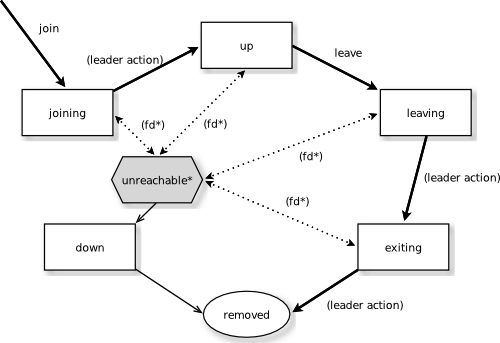
\includegraphics[width=0.7\textwidth]{membershipcluster.png}
\caption{Cluster membership states}
\label{fig:statescluster}
\end{center}
\end{figure}

In figure~\ref{fig:statescluster} the different states in which a cluster node
can be are illustrated. Alcaudon uses this mechanism in order to register new
nodes into the cluster using seed nodes. After joining the cluster, computation
nodes send a message to cluster coordinator in order to signal their
availability to receive new computations(\ref{code:noderegistering}).

\begin{lstlisting}[language=scala, frame=trBL, label=code:noderegistering, float=ht, caption = {Compute node registration}]
def register(member: Member): Unit =
    context.actorSelection(RootActorPath(member.address) / "user" / "coordinator") !
      ComputationNodeRegistration(member.id)
\end{lstlisting}

In order to shut-down nodes neatly, a protocol to leave Alcaudon clusters is
needed. This protocol is described in sequence diagram shown in
figure~\ref{fig:stopprotocol}.

\begin{figure}[!h]
  \centering
  \scalebox{0.45}{
    \input{figures/exitnode.latex}
  }
  \caption{Computation node stop protocol}
  \label{fig:stopprotocol}
\end{figure}

\subsection{Computation manager}

As exposed before, computation manager is responsible for deploying and
supervising computations and streams. In order to deploy computations and
streams, the addresses of each of them are needed. To accomplish this
goal, akka location transparency mechanism is used. Akka gives a logical address
to each actor deployed into the system. Having this address allows sending
messages between actors. The translation between the logical address and the
physical address is done transparently by akka. Once this detail is
clarified, deployment process will be described. Cluster Coordinator, as
described in previous subsections, schedules provided dataflow topologies among
the available computing nodes. First, cluster coordinator sends a request to a
computing node asking to deploy certain computations and streams. When the computing
node responds with an acknowledgment, the computation is deployed. The next
step is to start a ComputationExecutor actor for each computation in the request
as well as Stream actors. Once these actors have been started, their logical
addresses are communicated to other members that belong to the same dataflow via
\acs{CRDT}. Using this approach avoiding centralized knowledge for the location
of different computations allows better scalability and resilience. One of the
drawbacks of this approach is an increase in the complexity of ComputationExecutor
actors. Finally, computation manager sends back a message to the coordinator
informing that the deployment has finished. The whole process is represented as
a sequence diagram in figure~\ref{fig:librarymanagement}.

\begin{figure}[!h]
  \centering
  \scalebox{0.45}{
    \input{figures/deployment.latex}
  }
  \caption{Computation deployment sequence diagram}
  \label{fig:deployment}
\end{figure}

\subsection{Computation executor}

When computations are deployed, they are ready to process incoming records from
different sources and streams. One of the goals of the system is to provide
exactly once record processing semantics. In order to implement exactly once
semantics guarantees Alcaudon process records and timers in an idempotent
manner. The algorithm to provide these guarantees can be summarized as follows.

When a new record arrives into a computation the next steps are performed:
\begin{enumerate}
  \item Using duplication detection logic, records are checked to avoid duplicates.
  \item User defined code is run for the received record. This execution can
    result in pending changes to timers, state or downstream productions.
  \item Pending changes are saved into the database.
  \item An acknowledgment is sent back to senders.
  \item Pending new records are sent.
\end{enumerate}

Since storing the result of every new record processing could be costly, the
above operations can be grouped into batches optimizing the process. Records are
sent until the sender gets an acknowledgment, meaning that in reality records
are sent at least once, but the computations are idempotent.

\begin{lstlisting}[language=scala, frame=trBL, label=code:computationState, float=ht, caption = {Alcaudon internal computation state}]
case class ComputationState(kv: Map[String, Array[Byte]],
                              timers: Map[String, Timer],
                              bloomFilter: CuckooFilter[String],
                              var latestWatermark: Long = 0,
                              var processedRecords: Long = 0,
                              var failedExecutions: Long = 0)
\end{lstlisting}

In order to understand better how Alcaudon implements this logic, it will be
explained in depth. Alcaudon uses the actor model widely, computations are not
an exception. One powerful feature provided by Akka is persistent actors. This
extension enables stateful actors to persist their internal state so it can be
recovered in the case of a failure or a cluster migration. Alcaudon uses this
extension alongside with Apache Cassandra\footnote{Apple has a cluster with over
  75000 nodes storing 10 PB of data} as data store. User code can work with
persistent state, create timers or produce records using Alcaudon \acs{API}'s,
that generates state that should be handled by computation actors. Internal
state contains persistent state from the computations executed, timers and
meta-information(~\ref{code:computationState}). Each
deployed computation actor has an internal instance of
\lstinline[columns=fixed]{ComputationState}. Once a computation execution has
finished, it is possible it has pending data to be stored. These changes are wrapped
into a \lstinline[columns=fixed]{Transaction}, persisted using akka extension.
Once data has been saved into the backing storage, changes are applied into
\lstinline[columns=fixed]{ComputationState} and senders are
acknowledged~\ref{code:computationStateStorage}. During failure scenarios, stored
transactions will be re-materialized once the actor is restarted, this is
know as recovery process. This process could be costly, since it has to re-apply
every stored transaction. To decrease recovery time it is possible to take
snapshots of the state, therefore only transactions from that instant will be
re-applied during recovery phase. Alcaudon allows to configure the frequency in
which snapshots are taken. This behavior is almost identical to regular
databases, where transactions are stored into an append-only log, materialized into an
in-memory image of the system. Snapshots are taken frequently avoiding long
recoveries. This architectural pattern helps to build a fault-tolerant system
and it is easy to reason about.

\begin{lstlisting}[language=scala, frame=trBL, label=code:computationStateStorage, float=ht, caption = {Computation state persistence}]
case _: ComputationFinished =>
  persist(Transaction(pendingChanges)) { transaction =>
    applyTx(transaction, origin) // Transaction is materialized
    context.become(receiveCommand)
    cuckooFilter.put(runningRecordId) // Deduplication data is updated
    state.newProcessedRecord()
    clearPendingChanges()
    origin ! ACK(self, runningRecordId, 0l) // Senders are acknowledged
  }
\end{lstlisting}

As it has been illustrated, executed computations can lead to internal state
changes. This means that if a record is received more than once, a mechanism to
reject already processed records is needed. One solution could be to store every
single record \acs{UUID} into a database and check against that database for
every received record. This approach is quite simple, but it does not scale and
can lead to failures if the database is unresponsive. Alcaudon deals with this
problem using probabilistic data structures. Bloom filters are a space-efficient
probabilistic data structure used to test if an element is a member of a set.
Bloom filters have been used since the 1970s but there are newer data structures
such as Cuckoo Filters\cite{cuckoo} that outperform the former. Alcaudon uses
Cuckoo filters in order to detect duplicated records. One downside of these
probabilistic data structures is that they can return false-positives, meaning
that a record can be considered as it has been already processed. To solve this
issue, processed records \acs{UUID}s are stored into a cuckoo filter and
Cassandra. When the cuckoo filter considers that a record has been already
processed it is checked against the database. Taking into account that the total
probability of a false-positive is $2b/2^{f}$ where $b$ is the number of entries
per bucket and $f$ the fingerprint length in bits. The number of false-positives
is low and therefore the database accesses will be minimal.

\subsection{Timers}

Given the infinite nature of streaming processing, an instrument to
emit partial results is needed. Alcaudon implements timers as a mean
to produce partial results, a different solution to this problem could
be based on triggers. As it was stated in previous sections, the system
implements three types of timers:

\begin{itemize}
\item \textit{Fixed timers}
\item \textit{Recurrent fixed timers}
\item \textit{Watermark timers}
\end{itemize}


\begin{figure}
\centering
\begin{subfigure}{.5\textwidth}
  \centering
  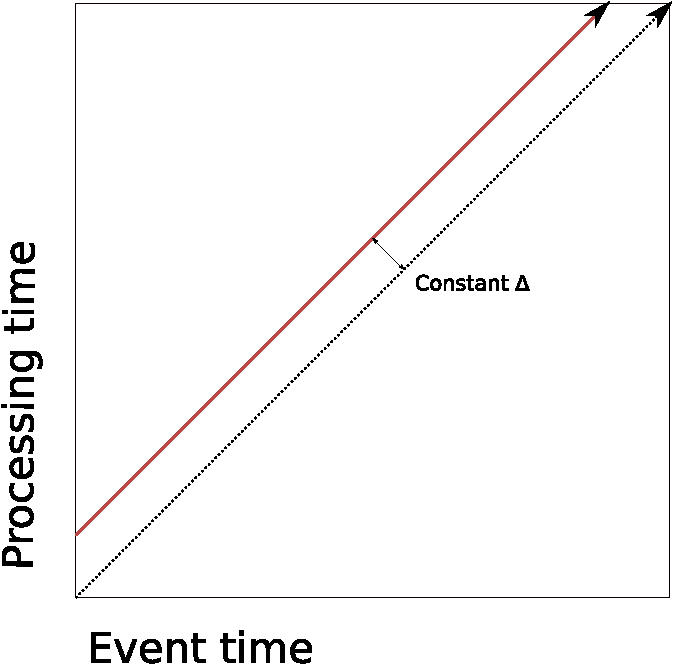
\includegraphics[width=0.8\linewidth]{constantskew.pdf}
  \caption{Constant time skew}
  \label{fig:constantskew}
\end{subfigure}%
\begin{subfigure}{.5\textwidth}
  \centering
  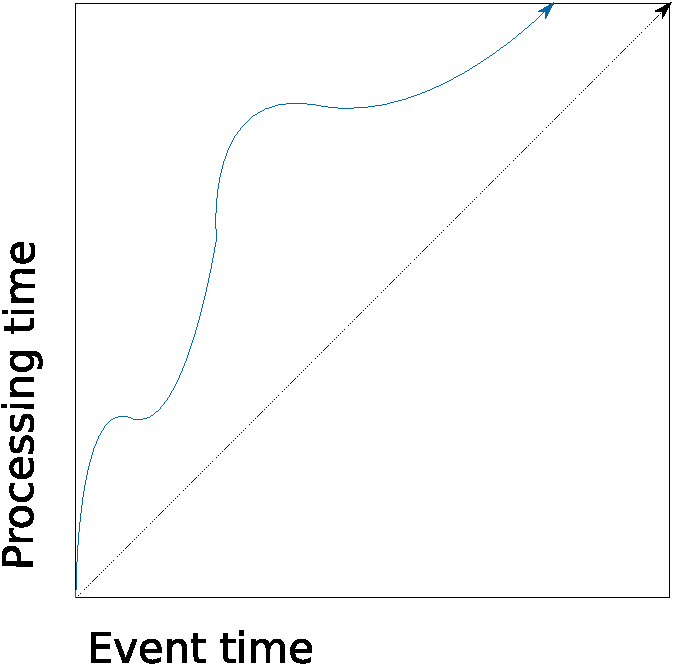
\includegraphics[width=.8\linewidth]{realskew.pdf}
  \caption{Irregular time skew}
  \label{fig:randomskew}
\end{subfigure}
\caption{Differences between ideal event time-process time skew and real world skew}
\label{fig:skew}
\end{figure}

Fixed timers are triggered based on system wall clocks, meaning that they do not
take into account event time. These timers are implemented using akka scheduler,
a system that allows scheduling message delivery between actors. They are a good
fit for computations that need to emit results at constant rate and do not need
a correlation with event times. However, there are occasions where it is needed
to know if events up to certain point in time have been processed. Due to the
nature of distributed systems it is difficult to know if at a given point in time,
all the events up to then have been received. In the ideal world, the
difference between event time and processing time would be a constant $\delta$ as
shown in figure~\ref{fig:constantskew}. Sadly, reality looks more
like figure~\ref{fig:randomskew}. Alcaudon tries to deal with this constraints
providing the grounds to work with and reason about out of order data. The choosen tool
is watermark timers, defined as follows:

\begin{definition}{Watermark}
Given a computation, $A$, let the oldest processed record in $A$ be a timestamp
corresponding to the oldest unfinished record in $A$.
Given this, watermark of $A$ is:
$min(oldest record of A, watermark of C : A depends on C)$
\end{definition}

Watermarks try to predict a timestamp $T_n$ signaling that up to that instant
all records have been received. Alcaudon implements a simple heuristic in order
to predict low watermarks. However more advanced techniques such us machine learning
can be used in order to predict low watermarks better. It is worth mentioning that this
very same algorithm was implemented by Google\cite{millwheel} and just about $0.001\%$
of records were dropped due to an incorrect prediction.
Therefore, using watermarks it is possible to configure timers that are
triggered once the watermark has reached a certain point, i.e. all records up to a
timestamp $T$ have been processed. 

In order to implement watermarks in Alcaudon, a system to replicate low
watermarks between different computations and streams is needed. One possible
option could be centralizing this knowledge in the cluster coordinator. The main
downside of this approach is that it could be a single-point of failure. Another
reason to avoid centralization is that watermarks are calculated in computation
basis, thus computations only need to have knowledge about their dependencies.
With this set of constraints \acs{CRDT}s are a good fit for the problem. They
are able to replicate changes among peers, they do not need coordination and
they provide eventual strong consistency. Again, akka provides an extension that
allows working with \acs{CRDT}s; akka distributed data. By default, this
extension provides different data type implementations such as counters, sets,
maps or registers. None of them are suitable to work with timestamps as is the
case of watermarks. Alcaudon implements a new \acs{CRDT} data type
\lstinline{GWatermark} that is able to satisfy the timestamps semantics as well
as \acs{CRDT} properties such as a monotonic merge function.
In Alcaudon, each \lstinline[columns=fixed]{ComputationExecutor} has a companion
actor, \lstinline[columns=fixed]{TimeExecutor}, who is in charge of keeping track
and triggering timers. This actor subscribes to \acs{CRDT} watermark changes that are
originated in computation dependencies(~\ref{code:timeExecutor}).

\begin{lstlisting}[language=scala, frame=trBL, label=code:timeExecutor, float=ht, caption = {TimerExecutor \acs{CRDT}s dependencies subscription}]
class TimerExecutor(computationId: String,
                    sources: Set[String],
                    initialWatermark: Long)
    extends Actor
    with ActorLogging {

      ...
  override def preStart(): Unit = {
    sources.foreach { srcId =>
      val key = GWatermarkKey(s"watermark-$srcId")
      replicator ! Subscribe(key, self)
      replicator ! Get(key, ReadMajority(2.seconds))
    }
  }
  ...
}
\end{lstlisting}

Once values from dependencies are known, the algorithm implementation to
calculate computation watermarks is straightforward(~\ref{code:watermarkUpdate}).

\begin{lstlisting}[language=scala, frame=trBL, label=code:watermarkUpdate, float=ht, caption = {Watermark update logic}]
def updateWatermarks(watermarkTimers: List[WatermarkTracker],
                     sourceWatermarks: Map[SourceID, Long],
                     timestamp: Long): Unit = {
  val minWatermarkSource =
    Try(sourceWatermarks.values.min).getOrElse(Long.MaxValue)
  latestWatermark = oldestComputationTimestamp.min(minWatermarkSource)
  val overdueTimers =
    watermarkTimers.filter(tracker => tracker.overdue(latestWatermark))
  val pendingTimers =
    watermarkTimers.filterNot(tracker => tracker.overdue(latestWatermark))
  val trackers = overdueTimers.map { tracker =>
    tracker.origin ! ExecuteTimer(tracker.timer)
    tracker.copy(lastWatermark = latestWatermark)
  } ::: pendingTimers
  context.become(working(trackers, sourceWatermarks))
}
\end{lstlisting}

Once watermarks are calculated, it is checked against the created timers if some
of them are past that point. If this is the case, a timer is
triggered(~\ref{code:watermarkUpdate}).

\subsection{Streams}

\begin{lstlisting}[language=scala, frame=trBL, label=code:recordstorage, float=ht, caption = {Stream record storage}]
case record: RawRecord =>
  val origin = sender()
  persist(RawStreamRecord(state.nextRecordSeq, record)) { event =>
    state.update(event)
    origin ! ReceiveACK(event.rawRecord.id)
    signalSubscribers(overwhelmedSubscribers)
    if (shouldTakeSnapshot)
      saveSnapshot(state)
\end{lstlisting}

In Alcaudon, streams represent the delivery instrument between different
computations. Computations subscribe to one or more streams and publish to zero
or more streams. As with computations, durability is a key part of streams,
meaning that during failure scenarios data published into a stream should be
recovered once the system is restarted. Streams are implemented as actors, and in
order to make them durable akka persistence has been used. As explained before,
with akka persistence it is possible to to store actor state. Alcaudon's streams
work largely as an append-only log, where computations or sources publish records
and they are delivered to subscribed computations. Each received record is
stored into a durable storage, in this case Cassandra. Internally, this
operation is done in batches, minimizing I/O overhead. This process is listed
in~\ref{code:recordstorage}. As it can be observed, stream publishers are
acknowledged when a record has been received. Again at least-once delivery
semantics are used to avoid any data loss. Once a record has been received,
pending records are sent to subscribers. A typical problem when implementing
publisher-subscriber systems is how to deal with slow-consumers. This is known as
flow control, and some patterns to solve this problem are listed below: 

\begin{itemize}
\item \textit{Back-pressure}: Consumers signal producers that they are able to
  process messages, defining message rate.
\item \textit{Managed queue pattern}: Where the consumer uses a bounded queue in
  order to store pending records.
\item \textit{Drop messages}: This pattern is an evolution of managed queue pattern. When
  the rate difference between producer and consumer is too big, messages are dropped.
  This pattern is biased towards system stability over correctness.
\item \textit{Throttling}: Throttle publisher output rate according to contracts
  with consumers.
\end{itemize}

Alcaudon deals with this problem using a hybrid approach. Stream actors store
the latest message offset acknowledged by each consumer. With this information, it
is possible to know an approximate consume rate for each consumer. A consumer is
considered overwhelmed when it has $n$ pending records to acknowledge, where $n$
is a configurable parameter. In order to avoid consumers instability, Alcaudon
streams stop sending messages to overwhelmed consumers for a while. To check if
consumers are able to handle new messages again, streams send them a record to
check if they are able to process it.They are taken out of quarantine if they
are able to handle it. This process is represented as a sequence diagram in
figure~\ref{fig:flowcontrol}.

\begin{figure}[!h]
  \centering
  \scalebox{0.5}{
    \input{figures/flowcontrol.latex}
  }
\caption{Alcaudon flow control sequence diagram}
\label{fig:flowcontrol}
\end{figure}

As described in previous sections, users should provide a key extraction
function. With this function, each record gets a key assigned. This allows to
parallelize computations using that key as a routing property. In particular,
Alcaudon uses consistent hashing in order to decide to which computation
executor a record should be delivered~\ref{fig:streamkeypart}. The number of
parallel computations is configurable as a global parameter in Alcaudon
settings.

\begin{figure}
  \centering
  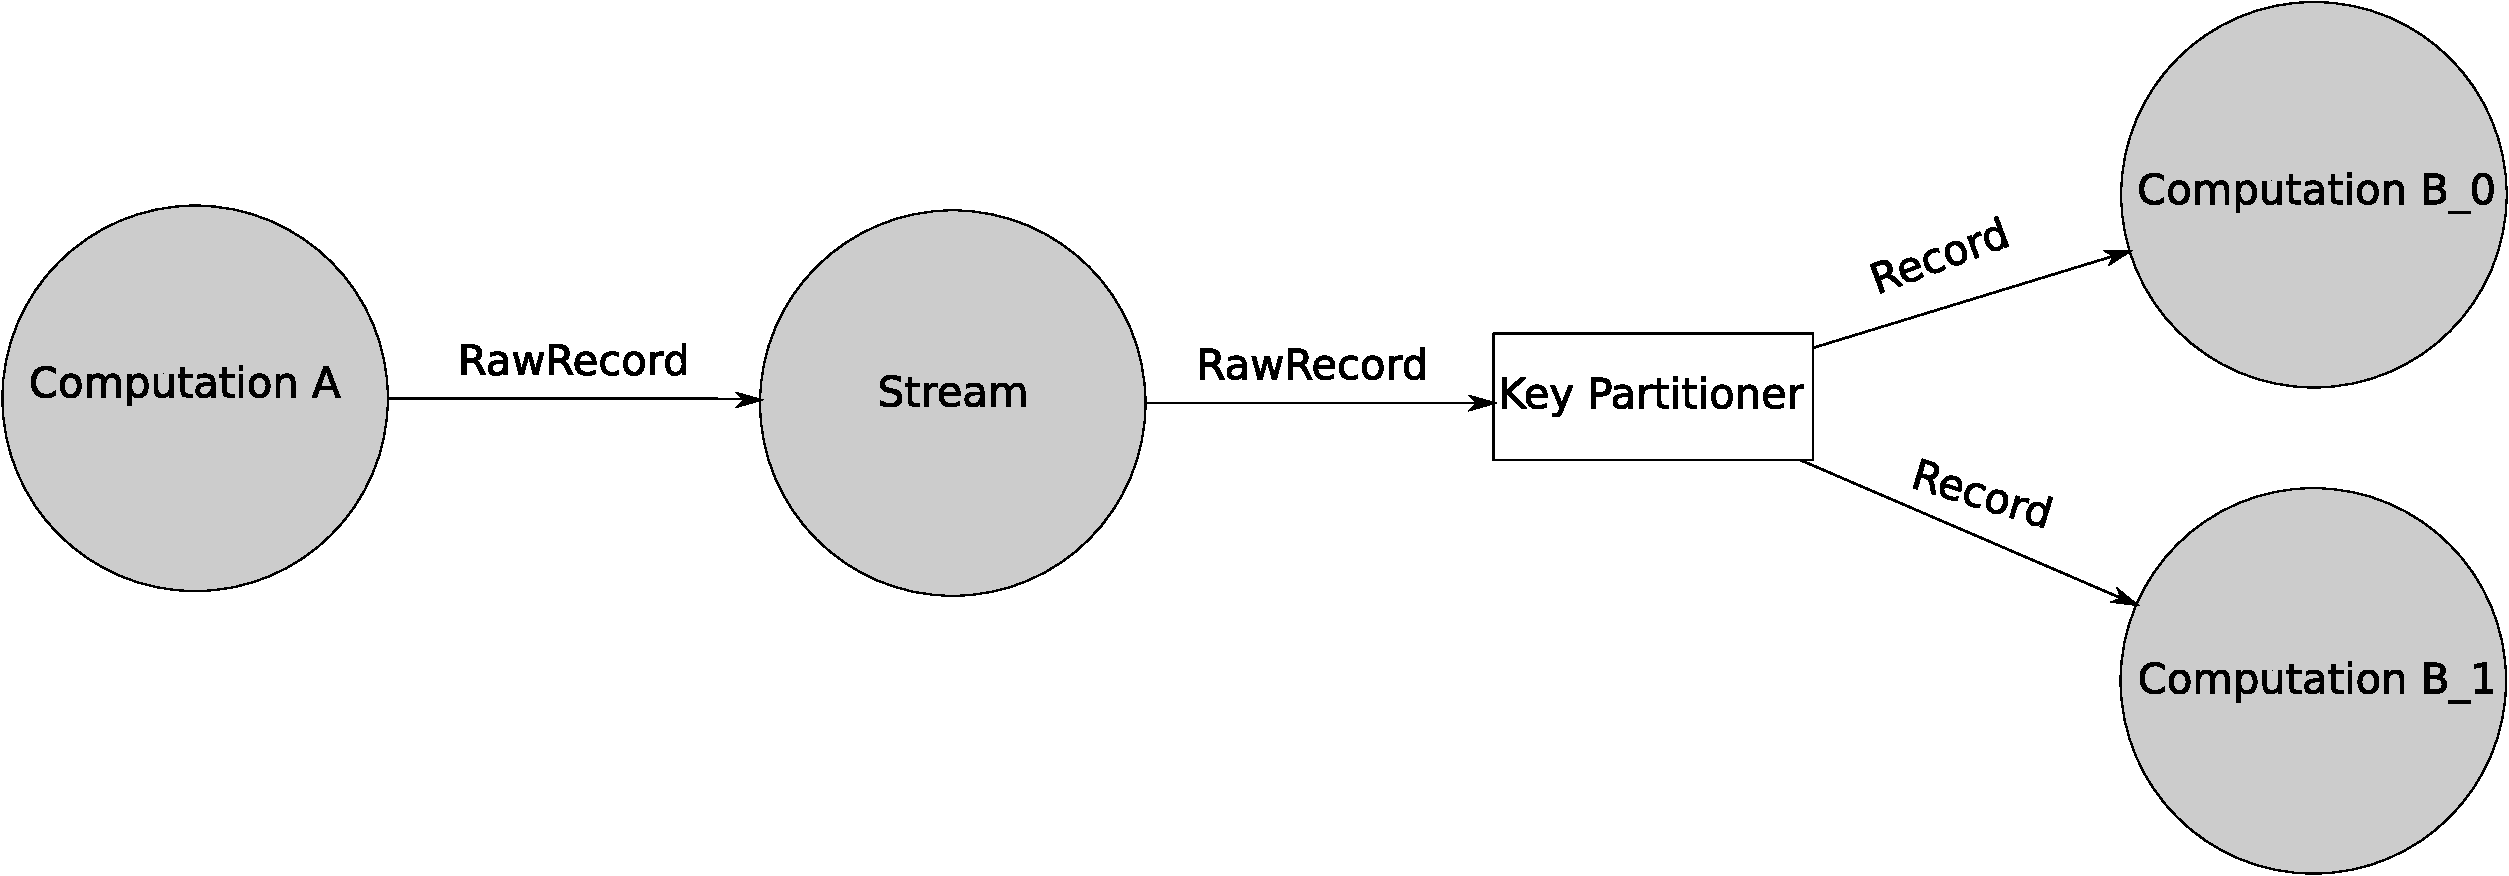
\includegraphics[width=0.8\textwidth]{stream.pdf}
  \caption{Streams key partitioning}
  \label{fig:streamkeypart}
\end{figure}

\section{Coordinator node}

Finally, coordinator node architecture design will be presented. This component
is in charge of keeping track of computation nodes, gathering different metrics,
creating new dataflow pipelines and scheduling them. A high level overview of this
system can be found in figure~\ref{fig:coordinatormodules}.

\begin{figure}[!h]
  \centering
  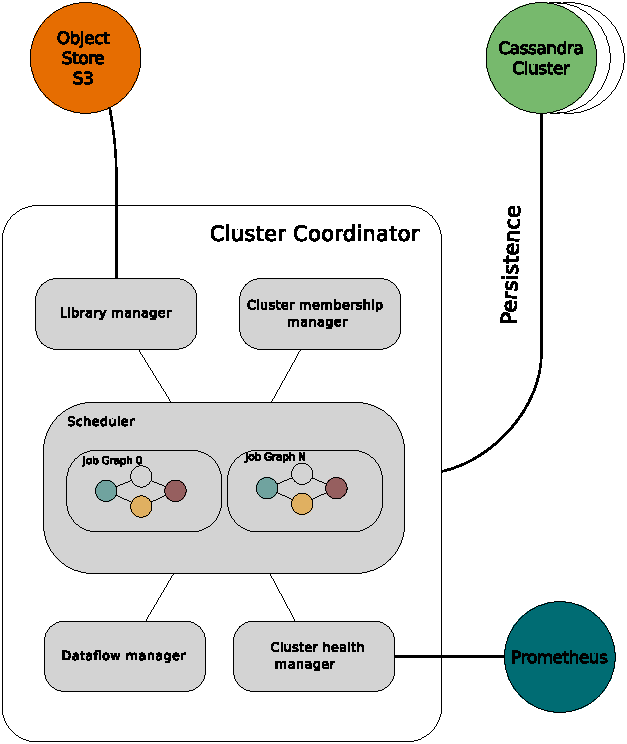
\includegraphics[width=0.6\textwidth]{coordinator.pdf}
  \caption{Coordinator node modules}
  \label{fig:coordinatormodules}
\end{figure}

Alcaudon coordinator node is composed of modules defined below:
\begin{itemize}
  \item \textit{Library manager}: It is in charge of storing user defined code
    into an object storage service.
  \item \textit{Cluster membership manager}: Module that manages the life-cycle of
    computing nodes in order to be able to schedule tasks in them.
  \item \textit{Dataflow manager}: Dataflow manager is the interface between
    users and the cluster. It defines how users create, monitor or destroy
    dataflow pipelines.
  \item \textit{Scheduler}: Scheduler is in charge of, given a dataflow pipeline
    to be deployed, get a deployment plan as optimal as possible.
  \item \textit{Cluster health manager}: This module is in charge of collecting
    different metrics such as CPU usage, memory usage, number of records
    processed, unhealthy nodes, etc. This nodes exposes an \acs{HTTP} interface
    so Prometheus is able to pull metrics data from it. It is used in
    combination with Grafana, a tool to generate time series dashboards.
\end{itemize}

Modules such as Library Manager and Dataflow Manager have been exposed in
previous sections, therefore this section will be focused on scheduling, cluster
membership manager, cluster health manager.

\subsection{Scheduler}

\begin{figure}[!h]
  \centering
  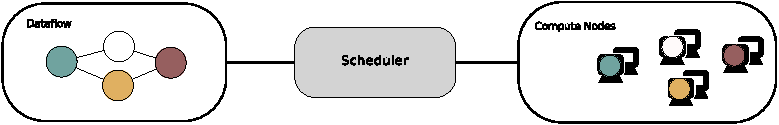
\includegraphics[width=0.8\textwidth]{scheduling.pdf}
  \caption{Scheduling process}
  \label{fig:scheduler}
\end{figure}

When dataflow pipelines are created, Alcaudon should deploy these computations
into available compute nodes~\ref{fig:scheduler}. Some desirable properties that
these deployments should have are:

\begin{itemize}
\item High cluster utilization
\item Fast job completion
\item Fairness
\item Efficiency
\end{itemize}

As it was described in previous sections, this problem is know as
\textit{flexible Job-shop scheduling problem} and it is cataloged as a NP-Hard
problem. Existing algorithms are based on heuristics and usually these
algorithms are biased towards fairness, performance or efficiency.
Alcaudon uses an state of the art cluster scheduler platform\cite{firmament},
named Firmament. It allows to use \acf{HTTP} in order to perform scheduling
requests. An interesting feature that this scheduler offers is that it allows
using different scheduling policies. These policies are listed below.

\begin{itemize}
\item \textit{Trivial}: Fixed costs, tasks always schedule if resources are idle.
\item \textit{Random}: Random costs, for fuzz tests.
\item \textit{SJF}: Shortest job first policy based on avg. past runtimes.
\item \textit{Quincy}: Original Quincy cost model, with data locality.       
\item \textit{Whare}: Implementation of Whare-Map's M and MCs policies.
\item \textit{Coco}: Coordinated co-location model.
\item \textit{Octopus}: Simple load balancing based on task counts.     
\item \textit{Void}: Bogus cost model used for KB with simple scheduler.  
\item \textit{NET-BW}: Network-bandwidth-aware cost model (avoids hotspots).  
\end{itemize}

After performing tests with different scheduling policies, Alcaudon uses
\textit{CoCo} scheduling policy as the defualt scheduling policy. It is
preferred to co-locate computations in order to save network round-trips.
However, it is possible to configure Alcaudon to use different policies.
Firmament calculations could take a long time, depending on the complexity
and \acs{DAG} to schedule size. In order to avoid long blocking \acs{HTTP}
requests, when a new scheduling request is performed, an operation code
is returned. With this code is possible to inspect how the operation is
evolving and eventually get a result. This process is summarized as as
sequence diagram in figure~\ref{fig:schedulefirmament}.

\begin{figure}[!h]
  \centering
  \scalebox{0.5}{
    \input{figures/schedulefirmament.latex}
  }
\caption{Sequence diagram for interaction between Firmament and Alcaudon}
\label{fig:schedulefirmament}
\end{figure}


\subsection{Cluster health manager}

Operating large distributed systems is challenging. In these environments,
multiple components are working together and eventually some of them could fail.
If the available tools to debug and monitor them are not adequate, finding a
problematic component could take hours. Given these facts, providing the tools
to monitor distributed systems is mandatory. One of Alcaudon's aims is to
provide metrics and mechanisms to deal with this problem. In order to implement
this feature, Prometheus has been used as a time series database and Grafana
as the dashboards generator. 

The component in charge of collecting metrics is \textit{cluster health
  manager}. This component listen to akka cluster events, in order to determine
the health from different nodes in the system. In also listen to some statistics
regarding actors, such as number of messages sent, mailbox size, CPU usage,
memory usage, statistics about jvm fork join pool,
etc(\ref{code:metricsSample}). All these metrics are stored into Prometheus,
allowing to query that times series data efficiently. Finally, Grafana consumes
data from Prometheus in order to graph different metrics.

\begin{lstlisting}[language=scala, frame=trBL, label=code:metricsSample, float=ht, caption = {Example of Alcaudon exposed metrics}]
# HELP akka_dispatcher_forkjoinpool_steal_count Akka ForkJoinPool Dispatcher Steal Count
# TYPE akka_dispatcher_forkjoinpool_steal_count gauge
akka_dispatcher_forkjoinpool_steal_count{dispatcherName="WebServer_akka.actor.default-dispatcher",} 49.0
# HELP akka_actor_group_processing_time Akka Actor Group processing time (Nanos)
# TYPE akka_actor_group_processing_time counter
akka_actor_group_processing_time{groupName="all",} 1.04116122E8
# HELP akka_router_processing_time_webserver_system_io_tcp_selectors Akka Router processing time (Nanos)
# TYPE akka_router_processing_time_webserver_system_io_tcp_selectors counter
akka_router_processing_time_webserver_system_io_tcp_selectors 2.541922E7
# HELP akka_router_error_count_webserver_system_io_tcp_selectors Akka Router errors
# TYPE akka_router_error_count_webserver_system_io_tcp_selectors counter
akka_router_error_count_webserver_system_io_tcp_selectors 0.0
# HELP akka_actor_group_mailboxes_size Akka Actor Group mailboxes size
# TYPE akka_actor_group_mailboxes_size gauge
akka_actor_group_mailboxes_size{groupName="all",} 1.0
\end{lstlisting}

Grafana~\ref{fig:grafana} allows to define custom dashboards and configure
alerts. Alerting is essential when monitoring distributed system. It is possible
to define alerts based on predictive models and warn system operators before
than the actual problem occurs, i.e. using simple linear regression for disk
size. An example for Alcaudon's domain could be, based on the growth of pending
dataflow pipelines to schedule, trigger an alert if that metric keep growing for
2 hours, meaning that the number of compute nodes is not enough.

\begin{figure}[!h]
\begin{center}
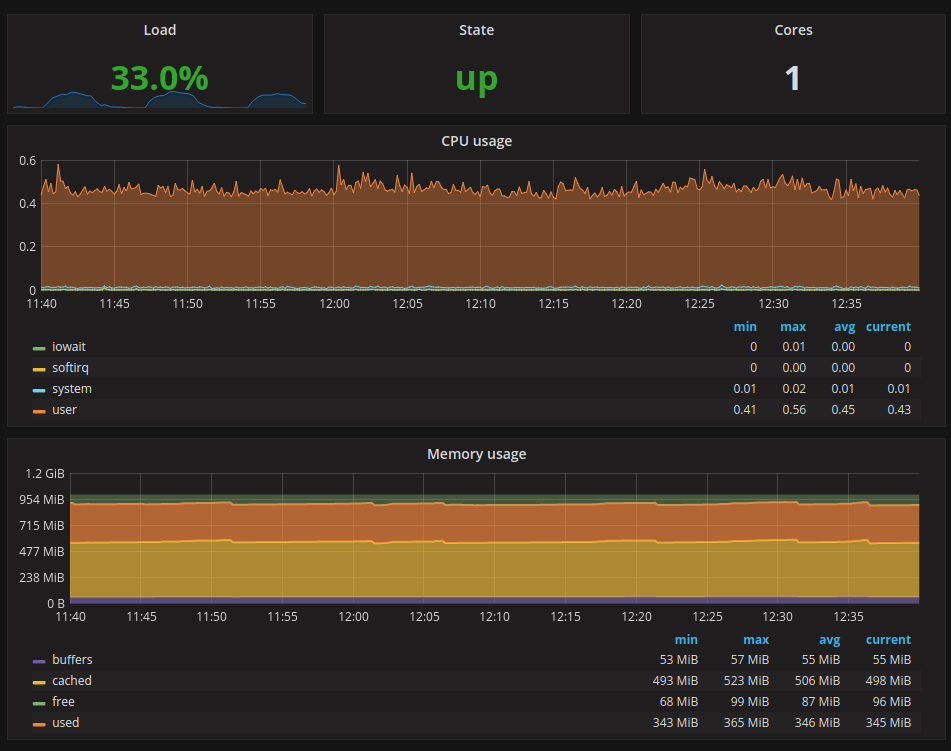
\includegraphics[width=0.7\textwidth]{grafana.png}
\caption{Grafana dasboard}
\label{fig:grafana}
\end{center}
\end{figure}

\section{Deployment}

In order to deploy the different components
